\chapter{技术指标}


\section{MACD}

% Ref: http://stockcharts.com/school/doku.php?id=chart_school:technical_indicators:moving_average_convergence_divergence_macd

以下内容来源于知乎\footnote{
作者:刘鹏程Sai.L \\
链接:https://www.zhihu.com/question/24114669/answer/26849139 \\
来源:知乎 \\
}。

顶背离就是区域A和区域B平均价格相差不大,甚至区域B的最高价高于区域A的最高价,但是
在与之相对应的MACD指标中a点与b点先后出现两个死叉,这两个死叉的相对位置和标的物价
位的相差成明显相反的效果。这一趋势性指标出现后,后市大跌的概率非常高。

{\color{red} MACD的顶背离在我国A股市场中是一个准确率极其高的趋势性指标。}



假设我是一个手握2亿资产的超级投资者,我看好一只总市值在4亿左右的股票,这一只股票
现在的价位是10元每股,我认为这个价格有拉升的空间,那么我就一直在用10元每股的价格,
一点点收集筹码。(当然,实际当中是不可能完全做到的,这里假设的是一个理想状态。)
当我完成了将2亿资金全部换成股票之后,我开始使用种种手段拉升这支股票的价格(具体
手段这里就不详细说了)。最后成功将价格拉升到了20元每股。那么现在我挣钱了么?答案
当然是没有,不仅没有挣钱,我还花掉了我所有的钱,看似2亿的盈利现在都只是一个账面
上的收益,想要真真正正拿到这2个亿的盈利,我必须把我手里的股票全部以20元每股的价
格卖掉。而且我不能一下子卖完,那样的话巨大的卖盘涌现,会使得股票价格快速下滑。我
需要很耐心的使用种种手段将价位稳定在20元每股左右,同时吸引其他人用真金白银将我手
里的股票买过去,把我手上的股票全部转化为现金,那么在盘面上就会看见一个价格高位震
荡一个比较长时间段的情况。当我将全部的股票转化为现金之后,这支股票的持有集中度就
显著下降,没有人刻意维持它的价格,不再有利好消息出现,当一些高位买入希望它进一步
上涨而获利的参与者开始失去耐心,想要卖掉这支股票开始调仓换股的时候,由于没有人托
价,股票价格将开始下跌。一旦下跌幅度加大,或者有利空消息出现,之前的跟风盘将踩踏
式出逃,价格将出现断崖式下跌。同时A股是个被操控性很强的市场,而且大多数股票被拉
升时都大幅超过本身应有价值,没有托盘的情况下,下跌都极为快速。所以MACD的顶背离在
A股市场上极其准确。如果在A股市场上你看见了一支股票在日线或者周线级别出现顶背离的
时候,那么请你立刻想象你自己就是阿甘,这个技术指标就是那个叫珍妮的小女孩,就是阿
甘的妈妈,阿甘在橄榄球场上的队友,阿甘在越战战场上的战友兄弟,他们都在朝你喊着同
一句话 Run,Forrest ! Run away !Hurry! 跑,快跑!不论你买入价位是多少,目前有
没有盈利。先跑出去再看,不要有任何心存侥幸和留恋。

-------------------------------------------

在A股市场中,底背离的正确率远远低于顶背离。再重复一遍,在A股市场中,底背离的正确
率远远低于顶背离。其原因在于,一支股票的价格能在高位长期徘徊而不下跌绝大多数都是
主力在维持这个价格,给出货争取时间这一种情况。而一支股票价格长期爬在地上不动就分
为俩种情况,一,有主力在刻意压制价格长期停留在一个较低的位置,方便于主力以低价收
集筹码。二,这支股票当中的主力全部,彻底的离开了,股价是被由于自身原因涨不上去,
也没有什么可跌的空间了,导致股价长期维持在一个价位。如果是情况二,那么你进入之后
可能很长一段时间都不会有什么像样的涨幅。那么怎么样才能增加顶背离这一信号的预测准
确率腻。

一,观察成交量。有主力介入进行低吸,并且后市将要进行拉升的股票,在低价区徘徊的时
期,成交量一定是温和放大的,因为无论怎样去抑制价格和演示自己进入的痕迹,为了获利,
买入行为时必然存在的,那么成交量上就会相交前期有所变化。

二,依靠时间跨度和指标的重复来增加判断正确率。在A股市场中俩个死叉形成的顶背离一
定要相信,俩个金叉形成的底背离一定要先观察,缓操作。底背离的组成里金叉越多,时间
跨度越大,可信度越高。


关于MACD就先讲到这里,这里特意要说一下,我用的MACD指标一般情况下都不是默认的
(12,26,9)而是改成了(10,20,5)。这么做的目的在于数值改小之后,指标效果会比默认数
值显示的效果超前一点点,同时,由于我选的三个参数都是5的倍数,显示出来的线条不像
默认数值那么圆润,而是比较锐利一点,这样交叉等重要情况在图形中看起来更加显眼。


\section{MA均线系统和BOLL布林带}
在我们通过趋势性指标寻找到一些上升趋势良好的股票之后,我们可以观察,也可以尝试去
买入一些,之后如果我们的判断没有大的漏洞的话。我们将看到这支股票的价格沿趋势开始
上涨。但是现在新的问题出现了,没有什么东西的价格会一直不停的涨下去,那么价格的波
动出现的时候,是短期的一个调整还是上涨结束了腻?有了盈利的股票需要什么时候思考出
售的问题?这里就需要借助一些压力与支撑类的指标。我个人寻找压力与支撑往往用均线和
布林俩个指标。当然在教科书上,他们俩个不是被定义为压力与支撑指标的。所以这里我讲
讲我的用法。

MA均线可能是所有指标中出现最早的一个指标了,只要一打开交易软件,它都会伴随着K线
图出现在我们眼前。它的原理简单到不能再简单,关于均线的运用也有无数的提法。可能是
太习以为常,我认识的很多人往往都关注那些一听起来就不明觉厉的指标,常常忽视了均线。


作者:水湄物语
链接:https://www.zhihu.com/question/24114669/answer/104567719
来源:知乎
著作权归作者所有。商业转载请联系作者获得授权,非商业转载请注明出处。

一位朋友被一段恋情折磨多年,那女人一次次欺骗他。虽然再跟这个女人维持关系,已经没有意义了,他还是一次次接受了她。
我问起他时,他说,他在这段感情里投入了这么多,现在却要放弃,是错误的。

电影很无聊,一个小时候,我跟朋友说,“走吧,我们回去吧。”她回答:“不行,不能白花这100块钱买电影票。”

以上是两个常见的纠缠沉没成本的例子。
继续纠结于沉没成本,只会让你付出更多的代价:再被那女人伤害几次,再浪费1小时在无聊电影上。同时,错过了寻找下一个好女人的机会。

股票投资者,经常成为沉没成本的受害者。
当他们看好的某只股票亏损之后,即便知道这只股票前景不妙,仍然抱住不放,不舍得斩仓出局。

这是不明智的,你过去赚了/亏了多少,一点都不重要。重要的是,股票未来的前景和走势。
要想摆脱这种谬误,需要理解为什么我们会纠结于沉没成本。

3) 短期记忆:
表现为我们更注重短期的记忆,而不是遥远的以前发生的事情。

人类的记忆力是非线性的,这已经被科学证实。
中国股市6000点的时候,有几个人还记得历次股灾——尽管随便打开一个资料,都能看到,历史上暴跌过N次。
但是……上个月大盘涨了15%噢!我的股票上周涨停了2次!……这些短期记忆,不断在洗刷我们的长期记忆。于是我们信心满满,认为眼前所见的一切将永久持续下去。

帕斯卡说过,人类的头脑既是宇宙的光荣,也是宇宙的耻辱。
其他误判包括:幸存者偏差、膀胱效应、心理锚定、风险厌恶、权威偏误……等等。

推荐书目:《清醒思考的艺术》。
这是一本很有趣的读物,可以避免你的思维被污染。


\section{布林线}

布林线是由美国交易者约翰布林格所创并且推广. 其主要的原理就是基本的概率分布: 先假
设价格会围绕一个均值上下波动, 然后利用统计标准差, 再根据概率分布理论来计算价格波
动的范围, 这个均值就是布林线的中轨, 而波动的范围就是布林线的上轨与下轨.

算法与参数设置

布林线的算法很简单, 我们先取一条中轨做基础, 原版的布林线选取的是20日简单移动平均
线, 然后我们再设定一个N倍标准差来做波动范围参数, 原版布林线设定的是2倍标准差, 最
后, 我们用中轨分别加减N倍标准差得出上轨与下轨, 从图表上看, 就是一个通道指标!

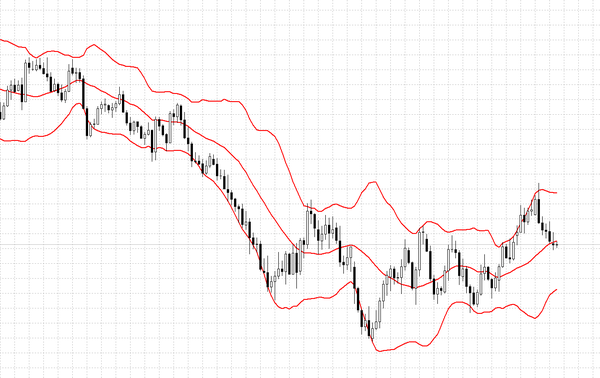
\includegraphics[width=\textwidth]{figure/boll1.png}

由于布林线有两个设置参数, 这样就决定了布林线有无数种变化! 我们既可以设置一条不同
参数的中轨(甚至还可以去编译一条中轨), 又可以选择不同倍数的标准差来做出上下轨!

不同的参数设置有着不同的应用方法, 这里只介绍一些最基本的用法!
1) 判断压力与支撑
当我们设置好布林线通道时, 第一个感觉就是价格大部分时间都在通道中波动, 这样, 我们
很自然地就认为布林线的上轨就是压力区, 布林线的下轨就是支撑区, 这是一种最常见的用
法. 如图

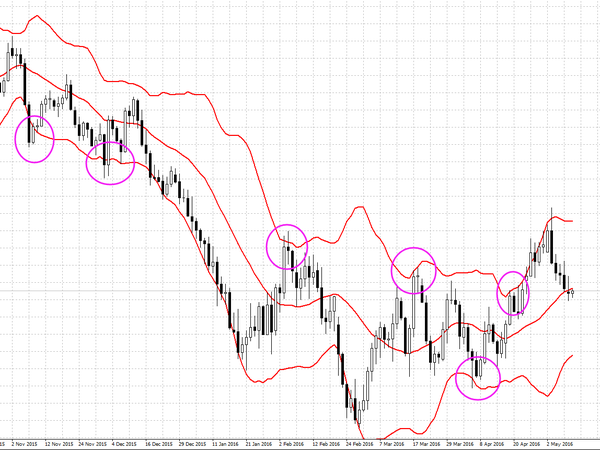
\includegraphics[width=\textwidth]{figure/boll2.png}

2) 识别趋势
布林线还有一个主要的用法是识别趋势. 使用布林线的交易者一般都会以中轨作为多空分界,
其实, 布林线还有一个特别重要的用法----行走在布林线上! 当价格波动到上下轨甚至超过
上下轨时, 价格很容易出现单边上涨或下跌的走势, 从布林线的形态上来看, 就是价格始终
都压在上轨或下轨上! 如图

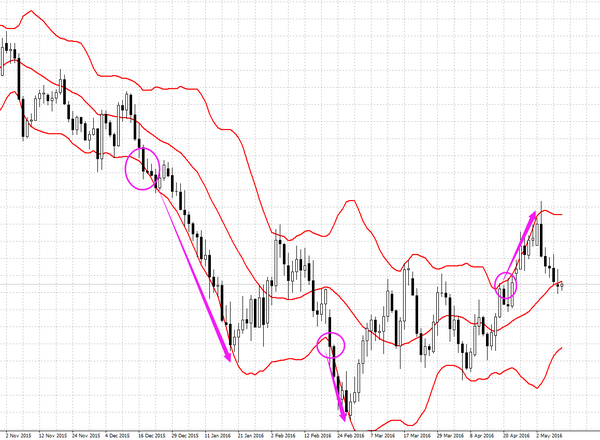
\includegraphics[width=\textwidth]{figure/boll3.png}

